\chapter{Learning Food Recognition Model with Deep Representation}\label{sec:cnn}

\section{Introduction}
Deep Learning with Convolutional Neural Networks (CNNs) is the most popular method for image recognition and has been applied to solve many real problems. In this chapter, we investigate problem of using the pre-trained CNNs for transfer learning. In particular, we fine-tune the parameters of the pre-trained CNNs on two food image database and achieve the improved results. We also investigate the changes of parameter after fine-tuning and try to obtain some important experience on fine-tuning the deep CNNs.
 



\section{Tuning the Deep CNNs}
The basic fact that fine-tuning can work for transfer learning is that Deep CNN can learn hierarchical features from bottom to top and some of the features are task-independent, especially most low-level and some mid-level ones.

There are two major strategies to fine-tune the deep CNNs: fine-tune the last layer (i.e. the classifier layer) and fine-tune the whole net.

\begin{itemize}
	\item \textbf{Fine-tune the last layer.} In the first strategy, we consider the deep CNNs as a fixed feature extractor and only modify the last layer of the net. This assumes that the features extracted by the pre-trained deep CNN can be directly applied to the new tasks. Therefore, by changing the last layer of the model, e.g. the combination of the features, the model can adopt new classes effectively. For example, when we introduce the mythical creature Sphinx to someone, we usually say it has the head of a human, the haunches of a lion, and the wings of a bird and people could obtain a rough idea of how Sphinx looks like without even see its picture. Here, the features such as head and haunches to describe Sphinx are high-level features that can be adopted directly from learned knowledge. Without learning from scratch, we can adopt the new concept effectively.
	\item \textbf{Fine-tune the whole net.} When fine-tuning the whole net, typically, we assume that some of the features extracted from the pre-trained deep CNN are not good enough for the new tasks. Therefore, we have to learn some new high-level features again. In fact, the high-level features are task-dependent and can be learned from those task-independent low-level features with certain combination. The purpose of fine-tuning the whole net is to changing the combination of the low-level features to reconstruct the task-dependent high-level features for the new task. 
\end{itemize}

For both strategies, the last layer, i.e. the layer of a classifier is removed. For different fine-tuning strategies, the error would back propagate to different layers (see Figure \ref{fig:ft-net}). Typically, a small learning rate is used to for fine-tuning the model to make sure that the model will not overfit the data of the target task.

\begin{figure}
	\centering
	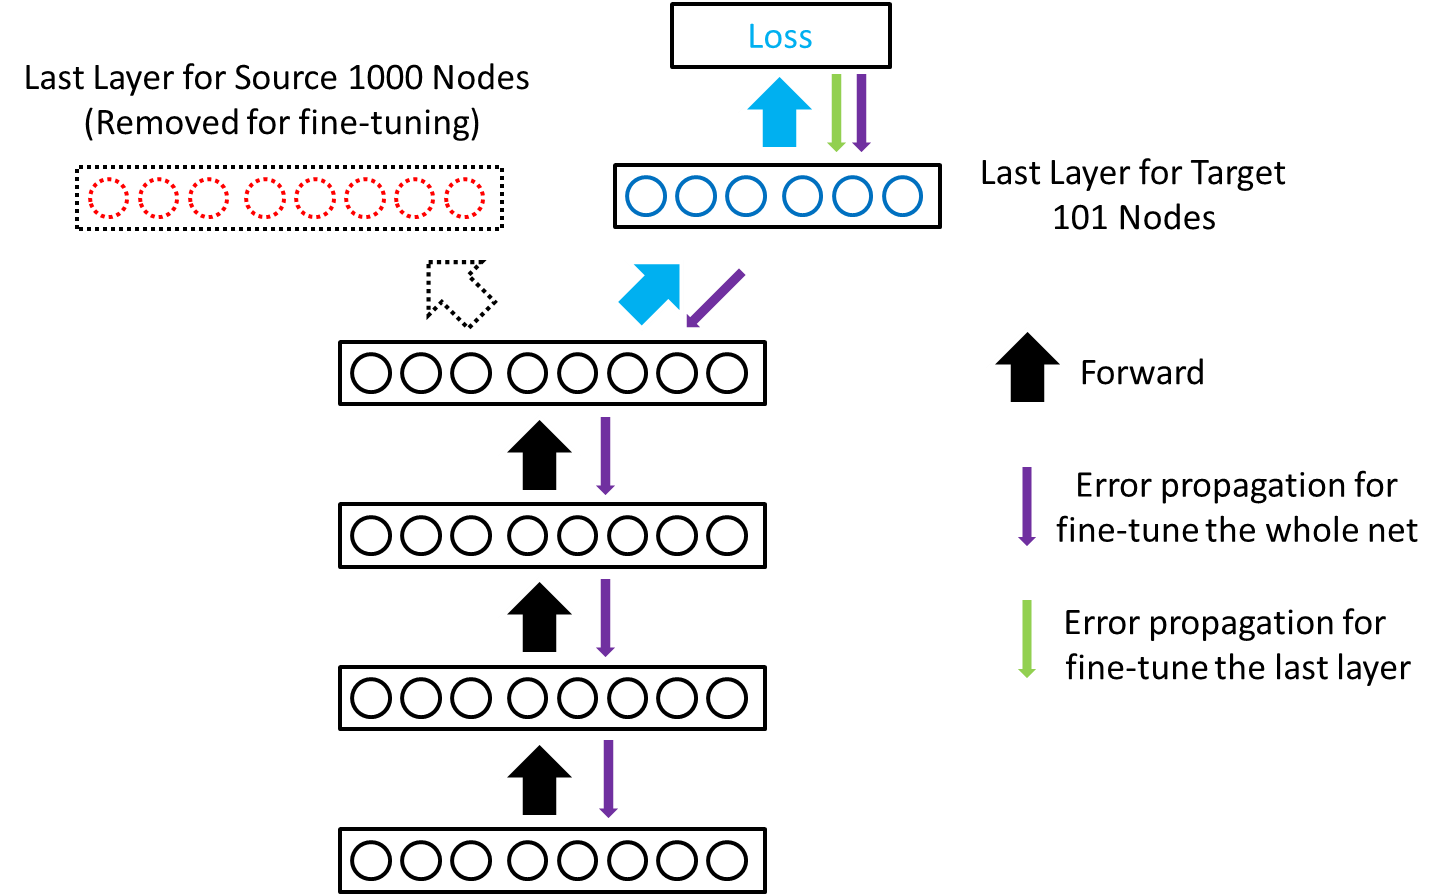
\includegraphics[scale=.5]{cnn/fig/ft.png}
	\caption{Demonstration of Fine-tuning from ImageNet 1000 classes to Food-101 datasets.}
	\label{fig:ft-net}
\end{figure}

\section{Layers in Deep CNN}
A CNN consists of some convolutional and subsampling layers optionally followed by fully connected layers. In this part, we introduce the layers used in our work.
\subsection{Convolutional Layer}
Convolutional Layer is the core building block of a Convolutional Network, and its output volume can be interpreted as holding neurons arranged in a 3D volume.
Natural images have the property of being "stationary" meaning that the statistics of one part of the image are the same as any other part. This suggests that the features that we learn at one part of the image can also be applied to other parts of the image, and we can use the same features at all locations.

Formally, given some original $h\times w$ input images $I$, we can train a small autoencoder from $a \times b$ kernel matrix. Also, we have to set other hyperparameters, stride $s$ and padding $p$. Stride defines the number of pixels the kernel should be moved in each step around the image $I$ and padding defines the number of rows/columns padded to the height and width of the original input (see Figure \ref{fig:cnn:conv}). 
Given a $a \times b$ kernel matrix $W^{(1)}$, bias $b^{(1)}$, padding $p$ and stride $s$, we can encode the original image $I$ as $f_{conv}=sigmod(W^{(1)}I_p+b^{(1)})$ for $I_p \in I$, giving us $f_{conv}$ (called feature map of $W^{(1)}$), a  $\left\lceil\frac{(h-a+2p)}{s}+1\right\rceil\times\left\lceil\frac{(w-b+2p)}{s}+1\right\rceil$ array of feature map. In general, for any specific input $I$ ($h \times w \times c$ array matrix) of a convolutional layer $L$, assuming we have $k$ such $a \times b \times c$ kernel matrix, its feature maps $f$ should be a $\left\lceil\frac{(h-a+2p)}{s}+1\right\rceil\times\left\lceil\frac{(w-b+2p)}{s}+1\right\rceil \times k$ array matrix with $f_{conv}^{(i)}=sigmod(W^{(i)}I_p+b^{(i)})$ for $I_p \in I$ and $i \in 1,\dots k$.

In real applications, small kernels ($3\times3$, $5\times5$ and $7\times7$) are preferred by many different CNN architectures \cite{krizhevsky2012imagenet} \cite{lecun1998gradient} \cite{simonyan2014very} \cite{zeiler2014visualizing}. Recent development of tiny $1\times1$ kernel shows an improvement on both accuracy and computational efficiency \cite{szegedy2014going}.
\begin{figure}
	\centering
	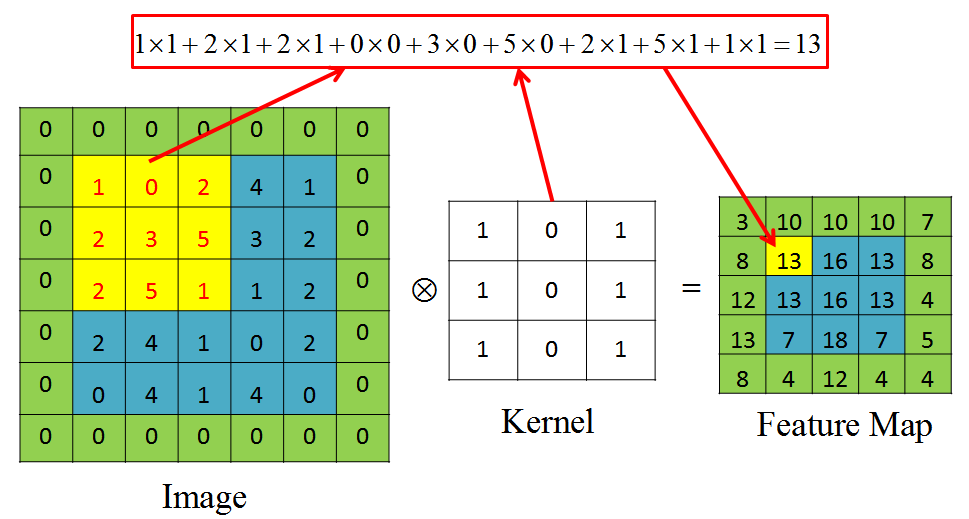
\includegraphics[scale=.6]{cnn/fig/conv.png}
	\caption{Convolution operation with $3\times3$ kernel, stride 1 and padding 1. $\otimes$ denotes the convolutional operator.} \label{fig:cnn:conv}
\end{figure}

\subsection{Pooling Layer}
Pooling layer is widely used in all kinds of CNN architecture for dimensional reduction and computational efficiency. 
After obtaining features maps using convolutional layer, we need to use them for classification. However, applying the feature maps from the convolutional layer for classification would be a computational challenge. Consider for instance images of size $96\times96$ pixels, and suppose we have learned 400 features over $8\times8$ inputs. Each convolution results in an output of size $(96-8+1)\times(96-8+1)=7921$, and since we have 400 features, this results in a vector of $892\times 400=3,168,400$ features per example. Learning a classifier from over 3 million features could lead to severe over-fitting.

Therefore, it is common to periodically insert a (Max) Pooling layer in-between successive convolutional layers in CNN architecture. Its function is to progressively reduce the spatial size of the representation to reduce the amount of parameters and computation in the network, and hence to also control overfitting. The pooling layer works independently on the channel dimension and resizes the feature map spatially. For certain $h \times w \times c$ input array matrix, a $a \times b$ Pooling layer with stride $s$ and $p$ padding would output a $\left\lceil\frac{(h-a+2p)}{s}+1\right\rceil\times\left\lceil\frac{(w-b+2p)}{s}+1\right\rceil \times c$ matrix array.

In general, two kinds of pooling strategy, Max Pooling and Average Pooling, are commonly used in CNN architecture (see Figure \ref{fig:cnn:pool}). Average pooling was often used historically but has recently fallen out of favor compared to the max pooling operation, which has been shown to work better in practice \cite{malmaud2015s} \cite{szegedy2014going}. Max Pooling is been widely used in all kinds CNN architectures \cite{boureau2010theoretical} \cite{yang2009linear}. 
\begin{figure}
	\centering
	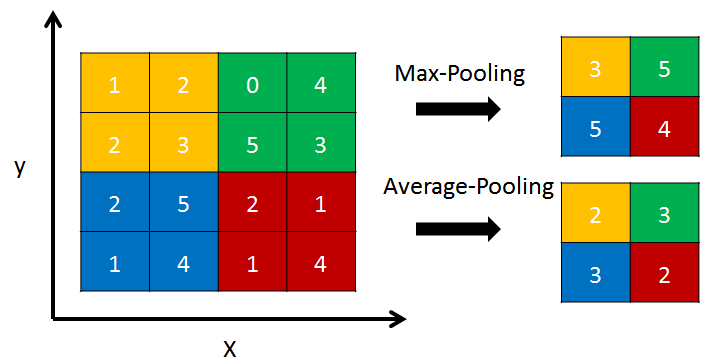
\includegraphics[scale=.8]{cnn/fig/pool.png}
	\caption{$2\times2$ pooling layer with stride 2 and padding 0.}\label{fig:cnn:pool}
\end{figure}

\subsection{Fully Connected Layer}
Fully Connected (FC) Layer have full connections to all activations in the previous layer, as seen in regular Neural Networks. Recent work show that FC layers with Rectified Linear Units and Dropout can greatly improve the learning speed as well as avoid overfitting for deep CNNs \cite{hinton2012improving} \cite{nair2010rectified}.
\subsubsection{Rectified Linear Units (ReLUs) for Activation}
Rectified Linear Units can be considered as replacing each binary unit with sigmoid activation by an infinite number of copies that all have the same weights but have progressively more negative biases. This replacing procedure can be mathematically presented as:
\begin{equation}
\sum\limits_i^N {\sigma (x - i + 0.5)}  \approx \log (1 + {e^x})
\end{equation}
where $\sigma(x)$ is the sigmoid function. In practice, Rectified Linear Units use the function 
\begin{equation}
f(x) = \log (1 + {e^x}) \approx \max(x,0) 
\end{equation}\label{eq:cnn:relu}
as the activation function for approximation \cite{jarrett2009best}. With $max$ function, the derivatives of the active ($x>0$) and inactive neurons are 1 and 0 respectively.  As a result, ReLUs can speed up the learning procedure greatly and improve the performance.
\subsubsection{DropOut}
In FC layer, nodes are connected to each other and this leads to a large number of parameters. Generally, larger number of parameters means more power for Neural Networks and more easily prone to overfitting. Dropout is a technique for addressing this problem.
The key idea is to randomly drop units (along with their connections) from the neural network during training \cite{srivastava2014dropout}. Technically, dropout can be interpreted as adding extra noise into the training procedure. Without actually adding noise, FC layer with dropout is tolerant of higher level of noise (20 \%-50\%). Randomly dropping out the nodes, for any node in FC layer, it can't rely on the other nodes to adjust its result. By eliminating the co-adaptation of hidden units, dropout becomes a technique that can be applied to any general domain and improve the performance of neural nets.   
\begin{figure}
	\centering
	\begin{tabular}{cc}
		\subfloat[ Standard Neural Net ]{    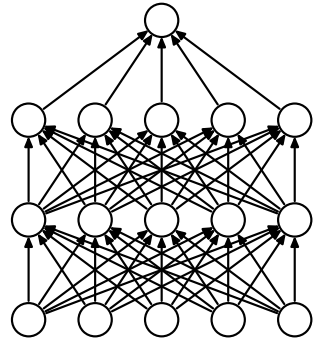
\includegraphics[width=0.3\textwidth]{cnn/fig/net.png}}&
		\subfloat[After Dropout]{    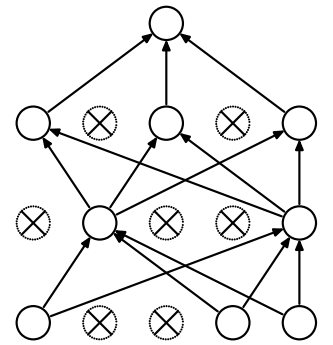
\includegraphics[width=0.3\textwidth]{cnn/fig/dropnet.png}} \\
	\end{tabular}
\end{figure}
\section{Datasets}
In this section, we introduce some details about the two architectures and the food datasets used in our experiments.
\subsection{Models}
In this paper, AlexNet and GoogLeNet are their Caffe \cite{jia2014caffe} implementations and all the results for a specific CNN architecture are obtained from a single model.

\textbf{AlexNet}
contains 5 layers followed by the auxiliary classifier which contains 2 fully connected layers (FC) and 1 softmax layer. Each of the first two layers can be subdivided into 3 components: convolutional layer with rectified linear units (ReLUs), local response normalization layer (LRN) and max pooling layer. Layer 3 and layer 4 contain just convolutional layer with ReLUs while layer 5 is similar to the first two layers except for the LRN. For each of the fully connected layer, 1 ReLUs and 1 dropout \cite{srivastava2014dropout} layer are followed.

\textbf{GoogLeNet}
shows another trend of deep CNN architecture with lots of small receptive fields. There are 9 Inception modules in GoogLeNet and Figure \ref{incept} shows the architecture of a single inception module. Inspired by \cite{linNiN}, lots of $1\times 1$ convolutional layers are used for computational efficiency. Another interesting feature of GoogLeNet is that there are two extra auxiliary classifiers in intermediate layers. During the training procedure, the loss of these two classifiers is counted into the total loss with a discount weight 0.3, in addition to the loss of the classifier on top. More architecture details can be found from \cite{szegedy2014going}.
%\begin{figure}
%\centering
%\includegraphics[scale=.11]{cnn/fig/g_v.pdf}\\
%\end{figure}
\begin{figure}
	\centering
	% Requires \usepackage{graphicx}
	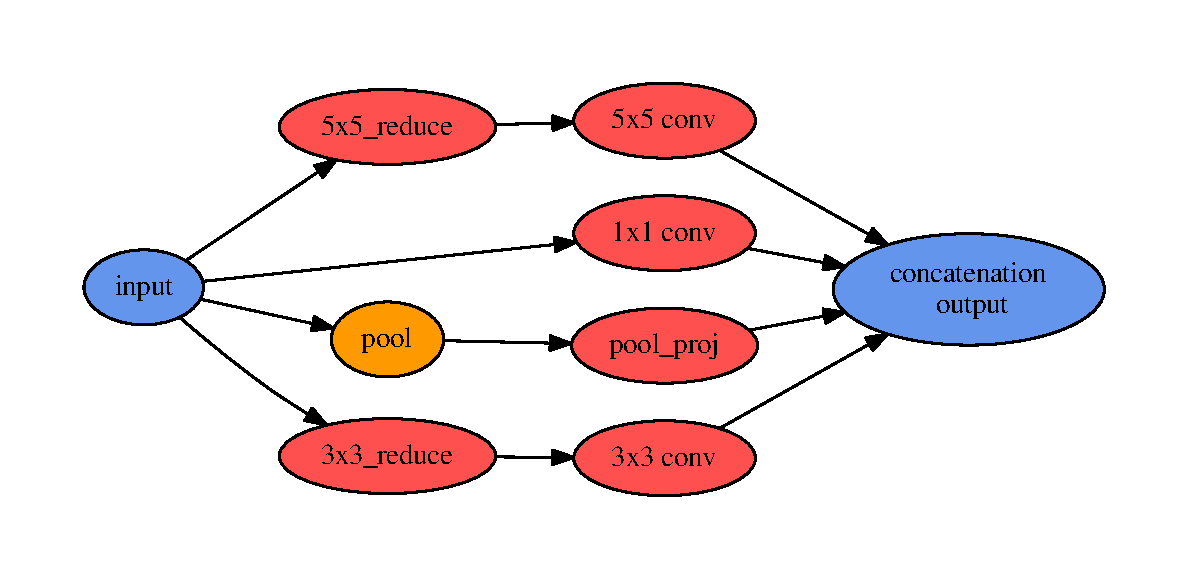
\includegraphics[scale=.7]{cnn/fig/inception.pdf}\\
	\caption{Inception Module. $n\times n$ stands for size $n$ receptive field, $n\times n\_reduce$ stands for the $1\times 1$ convolutional layer before the $n\times n$ convolution layer and $pool\_proj$ is another $1\times 1$ convolutional layer after the MAX pooling layer. The output layer concatenates all its input layers.}\label{incept}
\end{figure}

\subsection{Food Datasets}
Besides ImageNet dataset, there are many popular benchmark datasets for image recognition such as Caltech dataset and CIFAR dataset, both of which contain hundreds of classes. However, in this paper, we try to focus on a more specific area, food classification. Compared to other recognition tasks, there are some properties of the food (dishes) which make the tasks become a real challenge:
\begin{itemize}
	\item Food doesn't have any distinctive spatial layout: for other tasks like scene recognition, we can always find some discriminative features such as buildings or trees, etc;
	\item Food class is a small sub-category among all the categories in daily life, so the inter-class variation is relatively small; on the other hand, the contour of food varies depending on many aspects such as the point of view or even its components.
\end{itemize}
These properties make food recognition catastrophic for some recognition algorithms. Therefore, the training these two architectures on the food recognition task can reveal some important aspects of themselves and help people better understand them. In this paper, we use two image datasets Food-256 \cite{kawano14c}\footnote{Dataset can be found http://foodcam.mobi/dataset.html} and Food-101 \cite{bossard2014food}\footnote{Dataset can be found http://www.vision.ee.ethz.ch/datasets\_extra/food-101}. It is worthy to mention that PFID dataset is also a big public image database for classification, but their images are collected in a laboratory condition which is considerably not applicable for real recognition task.

\textbf{Food-256 Dataset.}
This is a relatively small dataset containing 256 kinds of foods and 31644 images from various countries such as French, Italian, US, Chinese, Thai, Vietnamese, Japanese and Indonesia. The distribution among classes is not even and the biggest class (vegetable tempura) contains 731 images while the smallest one contains just 100 images. For this small dataset, we randomly split the data into training and testing set, using around 80\% (25361 images) and 20\% (6303 images) of the original data respectively and keep the class distribution in these two sets uniform. The collector of this dataset also provides boundary box for each image to separate different foods and our dataset is cropped according to these boundary boxes.

\textbf{Food-101 Dataset.}
This dataset contains 101-class real-world food (dish) images which were taken and labeled manually. The total number of images is 101,000 and there are exactly 1000 images for each class. Also, each class has been divided into training and testing set containing 750 images and 250 images respectively by its collector. The testing set is well cleaned manually while the training set is not well cleaned on purpose. This noisy training set is more similar to our real recognition situation and it is also a good way to see the effect of the noise on these two architectures.

\subsection{Data Augmentation}
In this section, we introduce some data augmentation methods in our work to enrich our training data. Previous work shows that with intensive augmentation for the training data, the performance of CNN model can be improved \cite{wu2015deep}. 
Data Augmentation is an efficient way to enrich the data. There are also some techniques that can apply to enlarge the dataset such as subsampling and mirroring. The original images are firstly resized to $256\times 256$ pixels. We crop the 4 corners and center for each image according to the input size of each model and flap the 5 cropped images to obtain 10 crops. For the testing set, the prediction of an image is the average prediction of the 10 crops (see Figure \ref{fig:cnn:crop}).

\begin{figure}
	\centering
	\begin{tabular}{cccc}
		\multicolumn{2}{c}{\subfloat[Original image]{    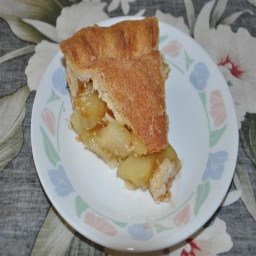
\includegraphics[width=0.15\textheight]{cnn/fig/crop00.png}}}&
		\subfloat[Center]{    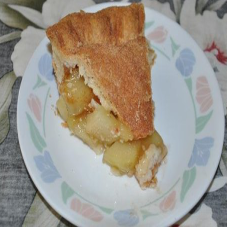
\includegraphics[width=0.15\textheight]{cnn/fig/crop4.png}}&
		\subfloat[Center mirror]{    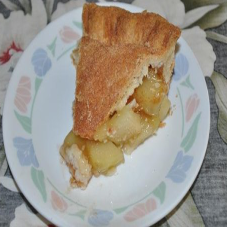
\includegraphics[width=0.15\textheight]{cnn/fig/crop9.png}}  
		\\    
		
		\subfloat[Up-left]{    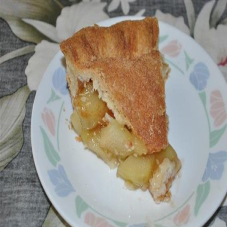
\includegraphics[width=0.15\textheight]{cnn/fig/crop0.png}}&
		\subfloat[Up-left mirror]{    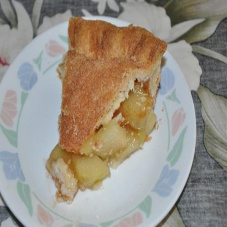
\includegraphics[width=0.15\textheight]{cnn/fig/crop5.png}} & \subfloat[Up-right]{    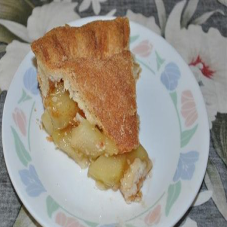
\includegraphics[width=0.15\textheight]{cnn/fig/crop1.png}}&
		\subfloat[Up-right mirror]{    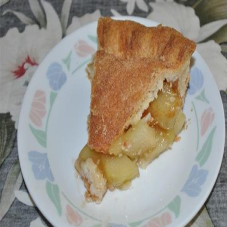
\includegraphics[width=0.15\textheight]{cnn/fig/crop6.png}}\\
		
		\subfloat[Bottom-left]{    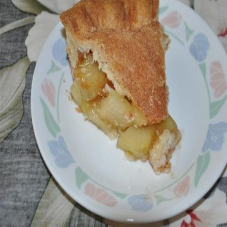
\includegraphics[width=0.15\textheight]{cnn/fig/crop2.png}}&
		\subfloat[Bottom-left mirror]{    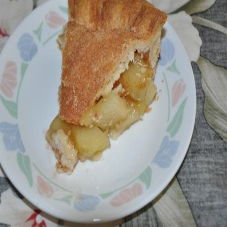
\includegraphics[width=0.15\textheight]{cnn/fig/crop7.png}} & \subfloat[Bottom-right]{    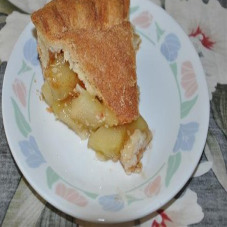
\includegraphics[width=0.15\textheight]{cnn/fig/crop3.png}}&
		\subfloat[Bottom-right mirror]{    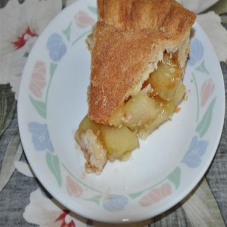
\includegraphics[width=0.15\textheight]{cnn/fig/crop8.png}}\\
		
	\end{tabular}
	\caption{Crop area from original image}\label{fig:cnn:crop}
\end{figure}

Before cropping subsamples from the original image, we also use other augmentation methods such as color casting and vignette etc., to enrich our data and make our model less sensitive to lighting changes and other invariance (see Figure \ref{fig:cnn:argu}). 

Compared to color shifting in \cite{krizhevsky2012imagenet}, we use color casting to alter the intensities of the RGB channels in training images. For each image, we firstly use a random boolean parameter to determine whether its R, G, and B channel should be changed. For any channel that should be changed, we add a random integer ranging from $[-20 , 20]$ to this specific channel. We also apply vignetting effect to the original image. In our implementation, we apply a 2D Gaussian kernel on the original image for vignetting. The two parameter $\sigma_x$ and $\sigma_y$ are randomly chosen from $[160,200)$. We also apply some geometric transformation such as stretching and rotation, on the original image for data augmentation. In summary, we enriched the data by 11 times, 3 times color shifting, 2 times vignetting, 4 times stretching and 1 time rotation and plus the original image.

During the fine-tuning process, we initial the learning rate 0.01 and it decreases 90\% (times 0.1) every 10000 iterations. The detail training configuration is shown in Table \ref{tab:config}.

\begin{figure}
	\centering
	\subfloat[Original image]{    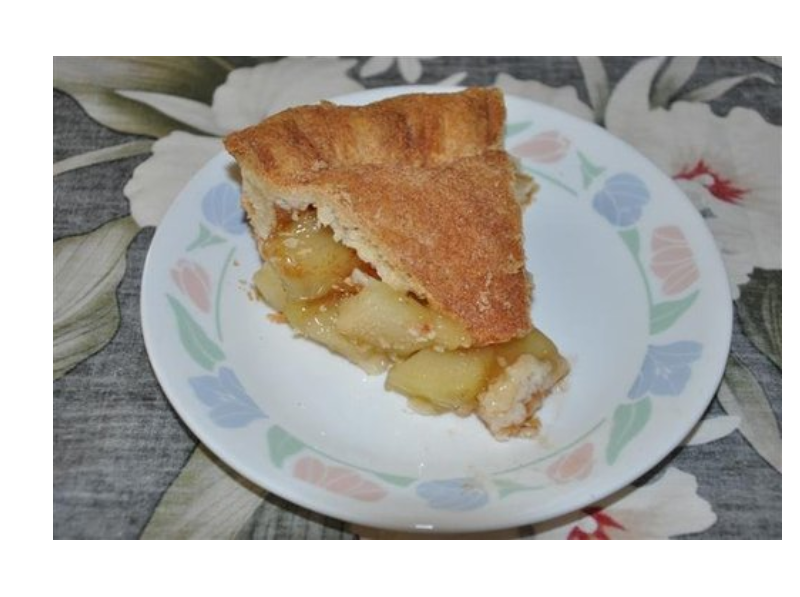
\includegraphics[width=0.3\textwidth]{cnn/fig/org.png}  }
	\subfloat[Red casting]{    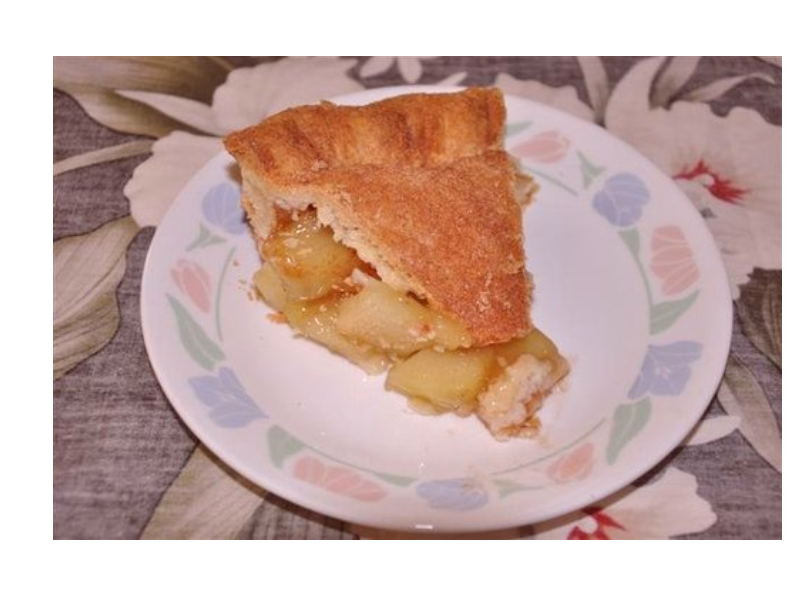
\includegraphics[width=0.3\textwidth]{cnn/fig/red.png}  }
	\subfloat[Green casting]{    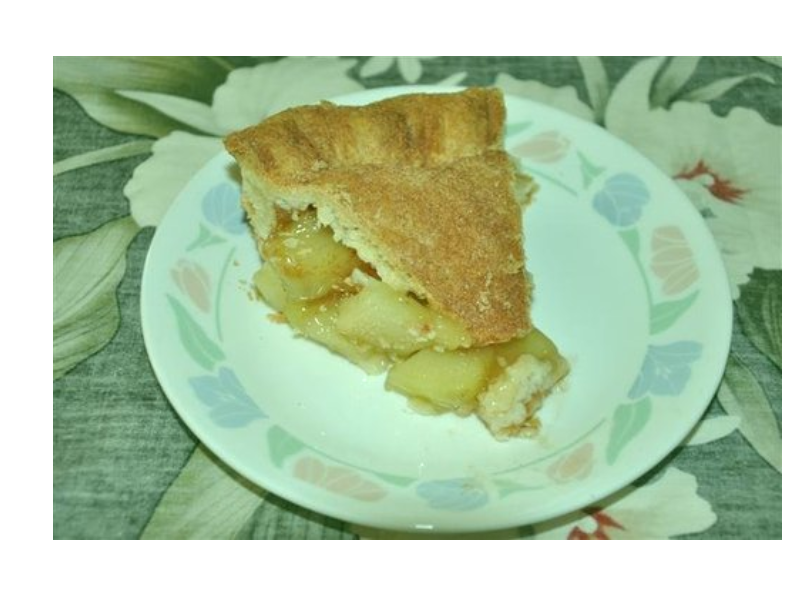
\includegraphics[width=0.3\textwidth]{cnn/fig/green.png}  }\\
	\subfloat[Blue casting]{    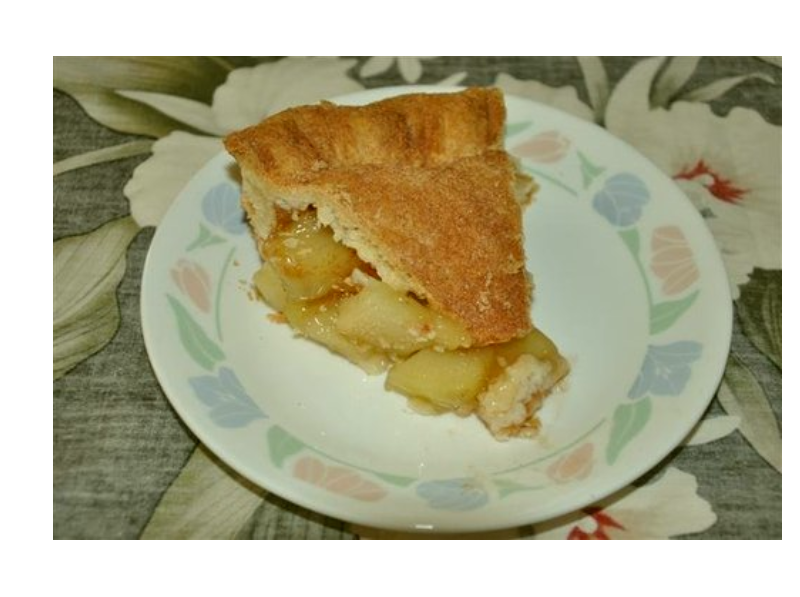
\includegraphics[width=0.3\textwidth]{cnn/fig/blue.png}  }
	\subfloat[RGB casting]{    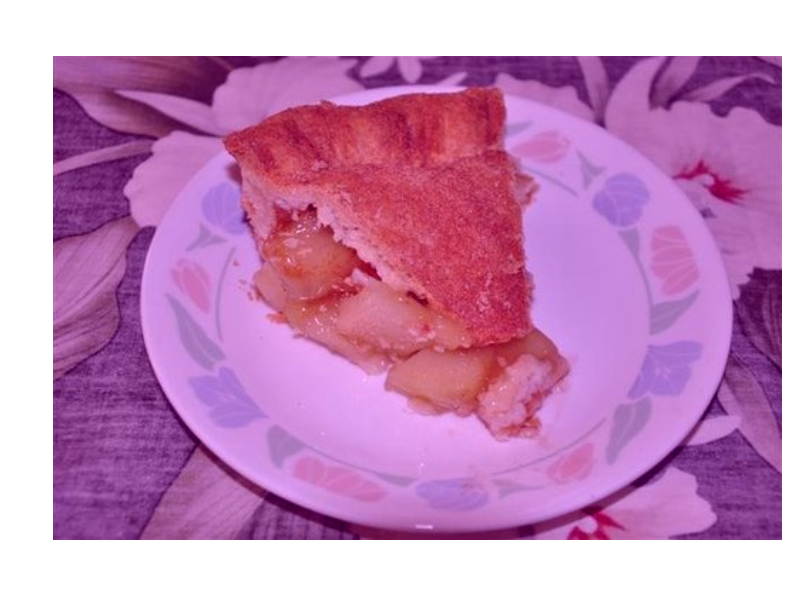
\includegraphics[width=0.3\textwidth]{cnn/fig/rgb.png}  }
	\subfloat[Vignette]{    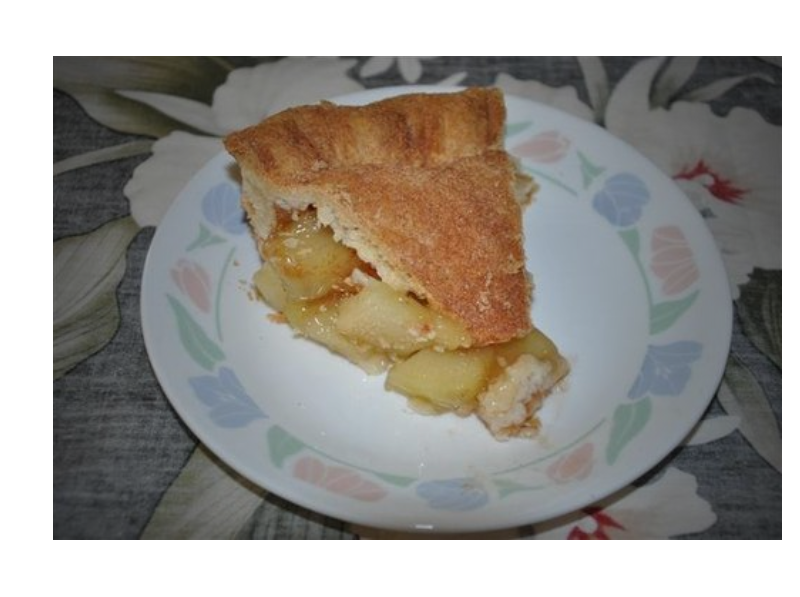
\includegraphics[width=0.3\textwidth]{cnn/fig/v1.png}  }\\
	\subfloat[More vignette]{    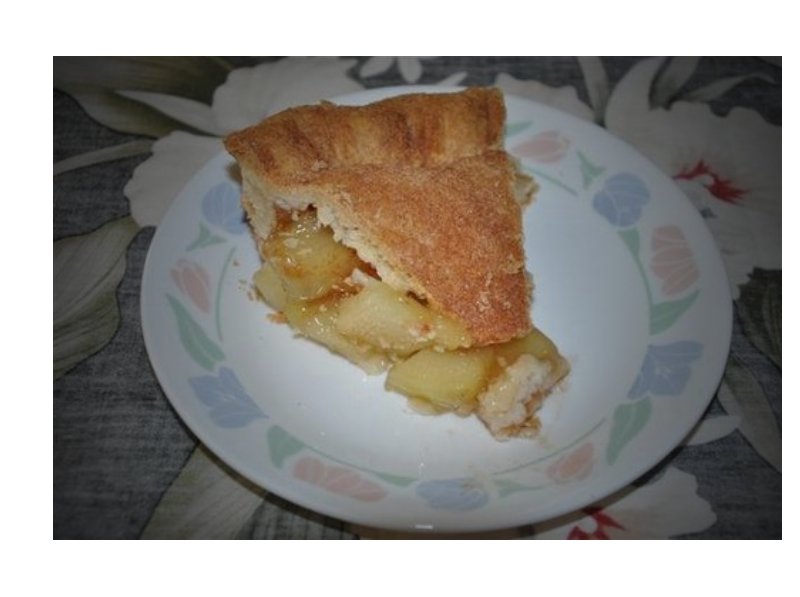
\includegraphics[width=0.3\textwidth]{cnn/fig/v2.png}  }
	\subfloat[Horizontal stretch]{    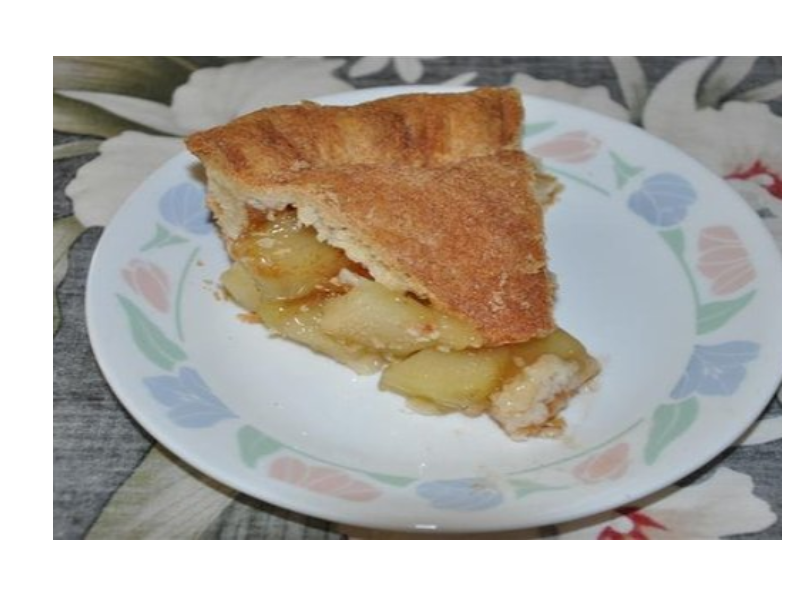
\includegraphics[width=0.3\textwidth]{cnn/fig/s1.png}  }
	\subfloat[More horizontal stretch]{    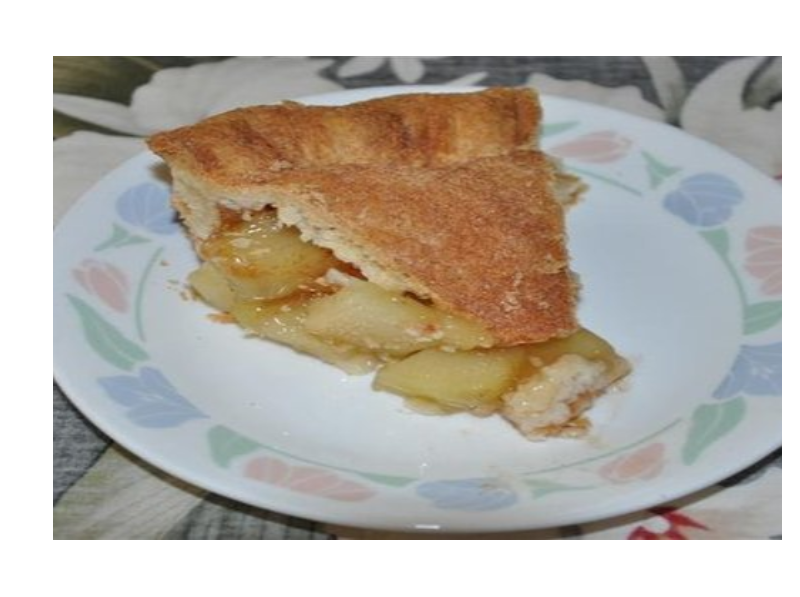
\includegraphics[width=0.3\textwidth]{cnn/fig/s2.png}  }\\
	\subfloat[Vertical stretch]{    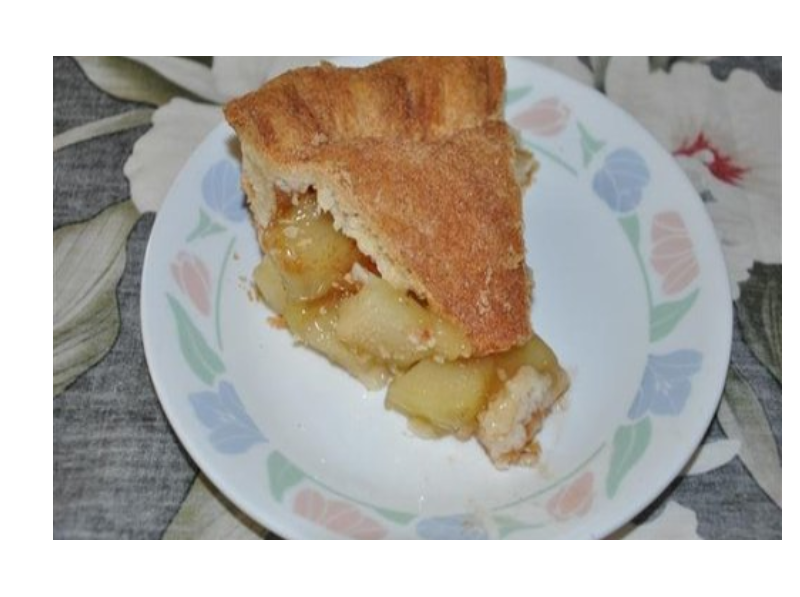
\includegraphics[width=0.3\textwidth]{cnn/fig/s4.png}  }
	\subfloat[More vertical stretch]{    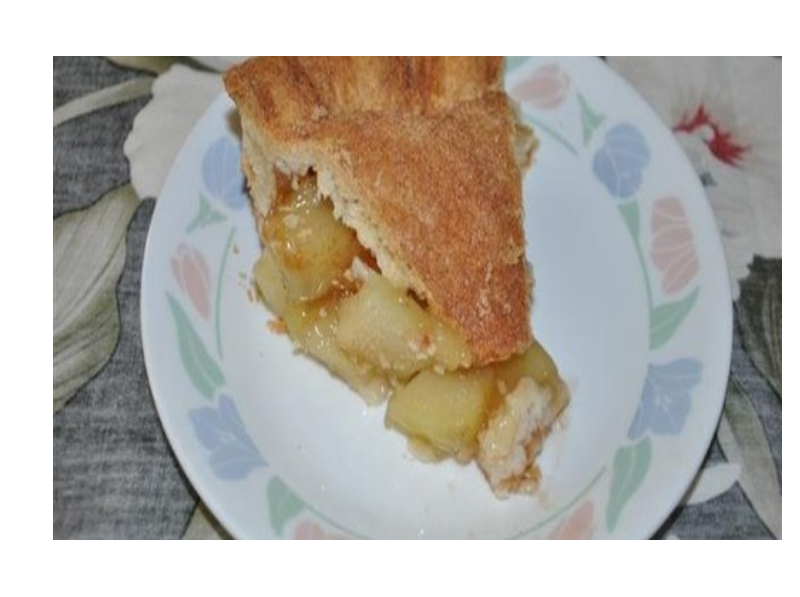
\includegraphics[width=0.3\textwidth]{cnn/fig/s3.png}  }
	\subfloat[Rotation]{    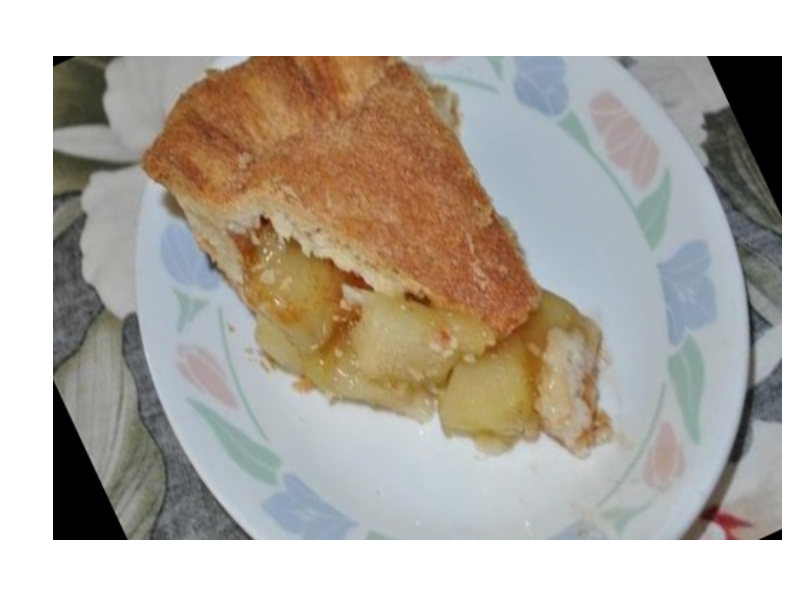
\includegraphics[width=0.3\textwidth]{cnn/fig/rota.png}  }\\
	
	\caption{Different data augmentation methods}\label{fig:cnn:argu}
\end{figure}


%\subsection{Configuration}
\begin{table}
	\centering
	\begin{tabular}{|c|c|}
		\hline
		Batch Size & 16 \\ \hline
		Learning Rate& 0.01\\ \hline
		Learning Rate Decay Policy& Drop 0.1 every 10000 iterations\\\hline
		Drop Rate & 0.1\\\hline
		Training Iteration& 100000\\\hline
		Momentum & 0.9\\\hline
		Weight Decay Rate& 0.0002\\\hline
		\end{tabular}
		\caption{Experimental configuration for GoogLeNet}\label{tab:config}
	\end{table}

\section{Experimental Discuss}
Training a CNN with millions of parameters on a small dataset could easily lead to horrible overfitting. But the idea of supervised pre-training on some huge image datasets could prevent this problem in a certain degree. Compared to other randomly initialized strategies with a certain distribution, supervised pre-training is to initialize the weights according to the model trained for a specific task. Indeed, initialization using the pre-trained model has certain bias as there is no single dataset including all the invariance for natural images \cite{agrawal2014analyzing}, but this bias can be reduced as the pre-trained image dataset increases and the fine-tuning should benefit from it.
\subsection{Pre-training and Fine-tuning}
We conduct several experiments on both architectures and use different training initialization strategies for both Food-256 and Food-101 datasets. The scratch models are initialized with Gaussian distribution for AlexNet and Xavier algorithm for GoogLeNet%, which automatically determines the scale of initialization based on the number of input and output neurons
\cite{glorot2010understanding}. These two initializations are used for training the original models for the ImageNet task. The ft-last and fine-tuned models are initialized with the weights pre-trained from the ImageNet dataset. For the ft-last model, we just re-train the fully connected layers while the whole network is fine-tuned for the fine-tune model.
\begin{table}[htbp]
	\centering
	\caption{Top-5 Accuracy in percent on fine-tuned, ft-last and scratch model for two architectures}
	\begin{tabular}{|l|cc|cc|}
		\hline
		& \multicolumn{2}{c|}{AlexNet} & \multicolumn{2}{c|}{GoogLeNet} \\  \hline 
		& Food-101   & Food-256   & Food-101   & Food-256 \\\hline
		Fine-tune & \textbf{88.12} & \textbf{85.59} & \textbf{93.51} & \textbf{90.66} \\\hline
		Ft-last &76.49    &79.26&    82.84    &83.77\\\hline
		Scratch & 78.18 & 75.35 & 90.45 & 81.20 \\\hline
	\end{tabular}%
	\label{tab:ft}%
\end{table}%


% Table generated by Excel2LaTeX from sheet 'Sheet1'
\begin{table}[htbp]
	\centering
	\caption{Accuracy compared to other methods on Food-256 dataset in percent}
	\begin{tabular}{|c|C{3cm}|c|c|}
		\hline
		& fv+linear \cite{Kawano:2014} & GoogLeNet & AlexNet \\\hline
		
		Top1  & 50.1& \textbf{70.13} & 63.82 \\\hline
		Top5  & 74.4  & \textbf{90.66} & 85.59\\\hline
	\end{tabular}%
	\label{tab:256}%
\end{table}%

% Table generated by Excel2LaTeX from sheet 'Sheet1'
\begin{table*}[htbp]
	\centering
	\caption{Top-1 accuracy compared to other methods on Food-101 dataset in percent}
	\begin{tabular}{|c|C{3cm}|C{3cm}|c|c|}
		\hline
		& RFDC\cite{bossard2014food} & MLDS($\approx$\cite{singh2012unsupervised}) & GoogLeNet & AlexNet \\\hline
		
		Top1 accuracy & 50.76 & 42.63& \textbf{78.11 }& 66.40 \\\hline
		
	\end{tabular}%
	\label{tab:101}
\end{table*}%
\begin{figure*}[htbp]
	\centering
	% Requires \usepackage{graphicx}
	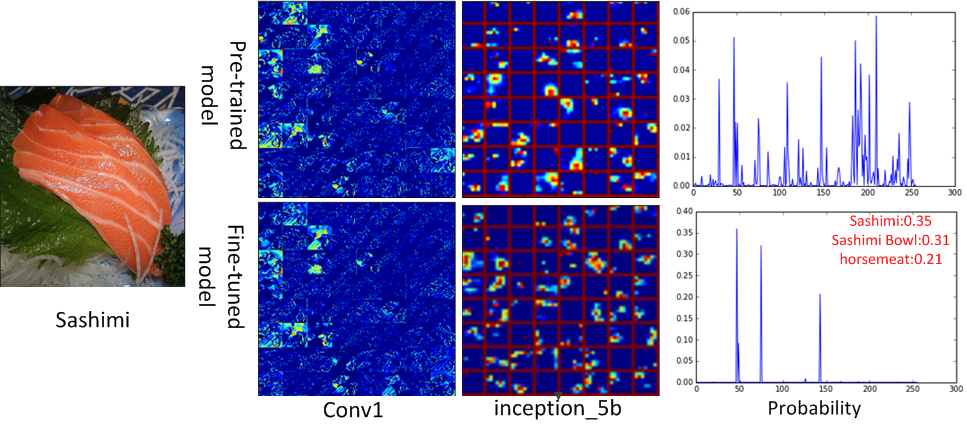
\includegraphics[scale=0.5]{cnn/fig/sashimi.png}\\
	\caption{Visualization of some feature maps of different GoogLeNet models in different layers for the same input image. 64 feature maps of each layer are shown. Conv1 is the first convolutional layer and Inception\_5b is the last convolutional layer. }
	\label{fig:sashimi}
\end{figure*}
From Table \ref{tab:ft} we can see that fine-tuning the whole network can improve the performance of the CNN for our task. Compared to other traditional computer vision methods (see Table \ref{tab:256} and \ref{tab:101}), GoogLeNet outperforms the other methods with large margins and we provide the state-of-the-art performance of these two food image datasets.

In Figure \ref{fig:sashimi} we visualize the feature maps of the pre-trained GoogLeNet model and fined-tuned GoogLeNet model with the same input image for some layers. We can see that the feature maps of the lower layer are similar as the lower level features are similar for most recognition tasks.
Then we can see that the feature maps in the high-level are different which leads to totally different recognition results.
Since only the last layer (auxiliary classifier) of the ft-last model is optimized, we can infer that the higher level features are more important which is consistent with our intuition. Also from Table \ref{tab:ft}, it is interesting to see that for the Food-101 task, the accuracy of the scratch models outperforms the pre-trained models. Since Food-101 is a relatively large dataset with 750 images per class while Food-256 dataset is an imbalanced small one, this indicates that it is difficult to obtain a good deep CNN model while the data is insufficient.

From Table \ref{tab:ft} we can see that GoogLeNet always performances better than AlexNet on both datasets. This implies that the higher level features of GoogLeNet are more discriminative compared to AlexNet and this is due to the special architecture of its basic unit, Inception module. Table \ref{tab:cosg} and \ref{tab:cosa} show the weights' cosine similarity of each layer between the fine-tuned models and their pre-trained models. From the results we can see that the weights in the low layer are more similar which implies that these two architectures can learn the hierarchical features. As the low-level features are similar for most of the tasks, the difference of the objects is determined by high-level ones which are the combination of these low-level features. Also from Table \ref{tab:cosa}, we can observe that the weights of the pre-trained and fine-tuned models are extremely similar in AlexNet. This can be caused by the size of receptive filed. Since ReLUs are used in both architectures, vanishing gradients do not exist. Rectified activation function is mathematically given by:
\begin{equation}\label{relu}
h = \max ({w^T}x,0) = \left\{ {\begin{array}{*{20}{c}}
	{{w^T}x}&{{w^T}x > 0}\\
	0&{else}
	\end{array}} \right.
\end{equation}

The ReLU is inactivated when its input is below 0 and its partial derivative is 0 as well. Sparsity can improve the performance of the linear classifier on top, but on the other hand, sparse representations make the network more difficult to train as well as fine-tune. The derivative of the filter is $\frac{{\partial J}}{{\partial w}} = \frac{{\partial J}}{{\partial y}}\frac{{\partial y}}{{\partial w}} = \frac{{\partial J}}{{\partial y}}*x$ where $\frac{{\partial J}}{{\partial y}}$ denotes the partial derivative of the activation function, $y=w^Tx$ and $x$ denotes the inputs of the layer. The sparse input could lead to sparse filter derivative for back propagation which would eventually prevent the errors passing down effectively. Therefore, the filters of the fine-tuned AlexNet is extremely similar. Compared to large receptive field used in AlexNet, the inception module in GoogLeNet employs 2 additional $n\times n\_reduced$ convolutional layers before the $3\times 3$ and $5\times 5$ convolutional layers (see Figure \ref{incept}). Even though the original purpose of these two $1\times 1$ convolutional layer is for computational efficiency, these 2 convolutional layers tend to squeeze their sparse inputs and generate the dense outputs for the following layer. We can see from Table \ref{tab:sparse} that the sparsity of the $n\times n\_reduce$ layers are denser than other layers within the inception module. This makes the filters in the following layer more easily to be trained for transfer learning and generate efficient sparse representations.
%\item The pooling strategy. In AlexNet, max pooling is applied to all the pooling layers between several convolution layers. During back propagation, the max pooling layer always passes the error to the place where it came from. Since it only came from one place of the receptive field, the back propagation error is sparse and keeps the most filters unchanged. In GoogLeNet, even though, there is a max pooling layer within every inception module, there are other 3 back-propagation errors, from $5\times 5\_reduce$ and $3\times 3\_reduce$ that can parse dense back-propagation errors to the previous inception module.


\begin{table*}[htbp]
	\centering
	\caption{Cosine similarity of the layers in Inception modules between fine-tuned models and pre-trained model for GoogLeNet}
	\begin{tabular}{|r|cccccc|}
		\hline
		\multicolumn{7}{|c|}{food256} \\\hline
		
		& \multicolumn{1}{l}{1x1} & \multicolumn{1}{l}{3x3\_reduce} & \multicolumn{1}{l}{3x3} & \multicolumn{1}{l}{5x5\_reduce} & \multicolumn{1}{l}{5x5} & \multicolumn{1}{l|}{pool\_proj } \\\hline
		inception\_3a & 0.72  & 0.72  & 0.64  & 0.67  & 0.73  & 0.69 \\
		inception\_3b & 0.59  & 0.64  & 0.53  & 0.70  & 0.60  & 0.56 \\
		inception\_4a & 0.46  & 0.53  & 0.54  & 0.50  & 0.67  & 0.38 \\
		inception\_4b & 0.55  & 0.58  & 0.63  & 0.52  & 0.69  & 0.41 \\
		inception\_4c & 0.63  & 0.64  & 0.63  & 0.57  & 0.68  & 0.52 \\
		inception\_4d & 0.60  & 0.62  & 0.60  & 0.58  & 0.68  & 0.50 \\
		inception\_4e & 0.60  & 0.61  & 0.67  & 0.61  & 0.68  & 0.50 \\
		inception\_5a & 0.51  & 0.53  & 0.58  & 0.48  & 0.60  & 0.39 \\
		inception\_5b & 0.40  & 0.44  & 0.50  & 0.41  & 0.59  & 0.40 \\  \hline
		\multicolumn{7}{|c|}{food101} \\ \hline
		& \multicolumn{1}{l}{1x1 } & \multicolumn{1}{l}{3x3\_reduce} & \multicolumn{1}{l}{3x3} & \multicolumn{1}{l}{5x5\_reduce} & \multicolumn{1}{l}{5x5} & \multicolumn{1}{l|}{pool\_proj } \\\hline
		inception\_3a & 0.71  & 0.72  & 0.63  & 0.67  & 0.73  & 0.68 \\
		inception\_3b & 0.56  & 0.63  & 0.50  & 0.71  & 0.60  & 0.53 \\
		inception\_4a & 0.43  & 0.50  & 0.50  & 0.47  & 0.62  & 0.36 \\
		inception\_4b & 0.48  & 0.52  & 0.57  & 0.50  & 0.67  & 0.35 \\
		inception\_4c & 0.57  & 0.61  & 0.59  & 0.53  & 0.63  & 0.47 \\
		inception\_4d & 0.54  & 0.58  & 0.53  & 0.54  & 0.64  & 0.44 \\
		inception\_4e & 0.53  & 0.54  & 0.61  & 0.55  & 0.62  & 0.42 \\
		inception\_5a & 0.43  & 0.47  & 0.53  & 0.45  & 0.57  & 0.34 \\
		inception\_5b & 0.36  & 0.39  & 0.46  & 0.38  & 0.52  & 0.37 \\
		\hline
	\end{tabular}%
	\label{tab:cosg}%
\end{table*}%


\begin{table*}[htbp]
	\centering
	\caption{Cosine similarity of the layers between fine-tuned models and pre-trained model for AlexNet}
	\begin{tabular}{|r|ccccccc|}
		\hline
		& conv1 & conv2 & conv3 & conv4 & conv5 & fc6   & fc7 \\
		\hline
		food256 & 0.997 & 0.987 & 0.976 & 0.976 & 0.978 & 0.936 & 0.923 \\
		food101 & 0.996 & 0.984 & 0.963 & 0.960 & 0.963 & 0.925 & 0.933 \\
		\hline
	\end{tabular}%
	\label{tab:cosa}%
\end{table*}%

% Table generated by Excel2LaTeX from sheet 'google'
\begin{table*}[htbp]
	\centering
	\caption{Sparsity of the output for each unit in GoogLeNet inception module for training data from Food101 in percent}
	\begin{tabular}{|r|cccccc|}
		\hline
		& 1x1  & 3x3\_reduce & 3x3  & 5x5\_reduce & 5x5  & pool\_proj  \\
		\hline
		inception\_3a & $69.3\pm 1.3$  & $69.6 \pm 1.1$  & $80.0\pm  1.0$& $64.1\pm  2.2$& $75.8\pm  1.6$& $76.2\pm 5.4$\\
		inception\_3b & $92.8 \pm 0.9$&$ 76.5 \pm 0.9$& $94.7\pm 0.9 $&$ 71.6 \pm 2.3 $&$ 94.4\pm 0.5 $&$ 94.7 \pm 1.6$\\
		inception\_4a & $90.9 \pm 0.9$& $70.0\pm 1.2 $& $93.8\pm 1.1 $& $63.3\pm 4.0 $& $91.9\pm 1.8 $& $95.1\pm 2.0$\\
		inception\_4b & $71.9 \pm 1.6$& $67.5\pm 1.2$ & $75.4\pm  1.0$& $58.5 \pm 2.6$& $78.9\pm  1.6$& $85.6\pm 3.6$\\
		inception\_4c & $75.1 \pm 2.4$& $72.6 \pm 1.3$& $81.0\pm 2.0$ & $66.3\pm 6.1 $& $79.7 \pm 3.6$& $88.1\pm 3.3$\\
		inception\_4d & $87.3 \pm 2.7$& $78.0 \pm 2.2$& $88.0\pm 1.6$& $67.9\pm 3.1 $& $88.9\pm 2.8 $& $93.0\pm 2.2$\\
		inception\_4e & $91.8\pm  1.1$& $62.3\pm 2.2 $& $91.0\pm 2.5 $& $49.5 \pm 3.7$& $94.0 \pm 1.0$& $92.3\pm 1.5$\\
		inception\_5a & $78.7 \pm 1.6$& $66.5\pm  1.7$& $82.3\pm 2.6 $& $59.9\pm 3.2 $& $86.4\pm 2.3 $& $87.1\pm 2.6$\\
		inception\_5b & $88.2\pm 2.3 $& $86.8 \pm 1.6$&$ 83.3\pm 4.4$ & $84.0\pm 3.1 $& $81.4\pm 5.3$  & $94.7\pm 1.5$\\
		\hline
	\end{tabular}%
	\label{tab:sparse}%
\end{table*}%

The unique structure of the Inception module guarantees that the sparse outputs from the previous layer can be squeezed with the $1\times 1$ convolutional layers and feed to convolutional layers with a bigger receptive field to generate sparser representation. The squeeze action promises the back propagation error can be transferred more efficiently and makes the whole network more flexible to fit different recognition tasks.

\subsection{Learning across the datasets}
From the previous experiments we can see that pre-training on the ImageNet dataset can improve the performance of the deep convolutional neural network in our specific area. In this part, we will discuss the generalization ability within the food recognition problem.  Zhou et al. trained AlexNet for Scene Recognition across two datasets with identical categories \cite{NIPS2014_Zhou}. But for more complex situation, such as two similar datasets with a little overlapped categories, we are very interested in exploring whether deep CNN can still successfully handle. Therefore, we conduct the following experiment to stimulate a more challenging real world problem: transferring the knowledge from the fine-tuned Food-101 model to a target set, Food-256 dataset. To make the experiment more practical, we limit the number of samples per category from Food-256 for training, because if we want to build our model using deep CNN for a specific task, the resource is always limited and it is exhausted to collect hundreds of labeled images for each category.

\begin{table*}[htbp]
	\centering
	\begin{tabular}{|c|cc|cc|}
		\hline
		& \multicolumn{2}{c|}{AlexNet} & \multicolumn{2}{c|}{GoogLeNet} \\
		\hline
		instances per class & ImageNet  & Food101\_ft    &  ImageNet  & Food101\_ft \\ \hline
		20    & 68.80  & {75.12} & 74.54 & {77.77} \\
		30    & 73.15 & {77.02} & 79.21 & {81.06} \\
		40    & 76.04 & {80.23} & 81.76 & {83.52} \\
		50    & 78.90  & {81.66} & 84.22 & {85.84} \\
		all    & 85.59 &  {87.21} & {90.66 }&   {90.65}     \\
		\hline
	\end{tabular}%
	\caption{Top5 Accuracy for transferring from Food101 to subset of Food256 in percent}
	\label{tab:cross}%
\end{table*}%

The Food-101 and Food-256 datasets share about 46 categories of food even though the images in the same category may vary across these two datasets. The types of food in Food-101 are mainly western style while most types of food in Food-256 are typical Asian foods. We compare the top-5 accuracy trained from different size of the subset for Food-256 on a different pre-trained model and the results are shown in Table \ref{tab:cross}.
%The ImageNet columns denote the pre-trained model trained only on ImageNet images and the Food101\_ft columns denote the pre-trained model trained on ImageNet images and then fine-tuned on Food-101.
The ImageNet columns denote using the model pre-trained from ImageNet dataset as the pre-trained model and Food101\_ft columns denote using the fine-tuned Food-101 model (the same one in Table \ref{tab:ft}) as the pre-trained model.

From the result of Table \ref{tab:cross} we can see that, with this further transfer learning, both CNNs can achieve around 95\% of the accuracy trained on full dataset while just utilizing about half of them (50 per class, 12800 of 25361 images). This indicates that when there is not enough labeled data, with its strong generalization ability, deep CNN trained from a general task can still achieve a satisfying result and perform even better when an additional relevant dataset is involved. This encouraging result may attract more people to use deep CNN for their specific task and continue to explore the potential of the existing architecture as well as designing new ones.



\section{Summary}
In this chapter, we show that fine-tuning GoogLeNet on two food databases can effectively transfer the knowledge from the general image recognition task to some specific recognition tasks. Without using any information of the source data, fine-tuning the deep CNNs on the target data shows impressive results. By comparing the changes of the parameters in each layers, we found that the high-level features can be easily changed while most low-level features are kept in fine-tuning.